\documentclass{article}
\usepackage{graphicx}
\usepackage{geometry}
\usepackage{listings}
\usepackage{hyperref}

 \geometry{
 a4paper,
 total={210mm,297mm},
 left=20mm,
 right=20mm,
 top=20mm,
 bottom=20mm,
 }
 
\begin{document}

\begin{center}
\textbf{\bfseries\Large ASSIGNMENT NO. 3}
\\[1cm]
\end{center}


\section{Aim : } 
	Write a mobile smart App to call a emergency land-line number/ mobile number using gyroscope/ iris
recognition/ thumb recognition or alike features of smart phone


\section{Objective : }  
	\begin{itemize}
		\item To understand Android Operating System.
		\item To implement Mobile Application Using Android OS.
	\end{itemize}

\section{Software Requirement : }  
	\begin{itemize}
    	\item Java Development Kit (JDK)
		\item Android Studio IDE
		\item Android Operating System
	\end{itemize}

\section{Mathematical Model : }  
	Consider a set S consisting of all elements related to a program. 
	The mathematical model is given as below.  \\  \\
    $S=\{input,output,function,success,failure\}$
	\begin{itemize}
		\item Input  :
			\begin{enumerate}
				\item Emergency Number
			\end{enumerate}
		\item Output :
        	\begin{enumerate}
				\item Store the emergency number
                \item Display the stored emergency number
			\end{enumerate}
		\item Function :
			\begin{enumerate}
				\item storeEmergencyNumber()
   				\item callEmergencyNumber()
			\end{enumerate}
		\item Success : Call the selected emergency number
        \item Failure : No such situation
	\end{itemize}  

\section{Algorithm : }
	\begin{itemize}
		\item Start
        \item Accept emergency name and number
        \item Store the emergency name and number
        \item Select the emergency contact
        \item Dial the selected contact
        \item Stop
	\end{itemize}


\section{Theory : }
 	
\subsection{Android:}
	\begin{itemize}
		\item Android is an open source mobile operating system (OS) currently developed by Google, based on the Linux kernel and designed primarily for touchscreen mobile devices such as smartphones and tablets
        \item Android was built from the ground-up to enable developers to create compelling mobile applications that take full advantage of all a handset has to offer. It was built to be truly open
        \item Android has an active community of developers and enthusiasts who use the Android Open Source Project (AOSP) source code to develop and distribute their own modified versions of the operating system
        \item Android provides access to a wide range of useful libraries and tools that can be used to build rich applications. Also includes a full set of tools that have been built from the ground up alongside the platform providing developers with high productivity and deep insight into their applications.
	\end{itemize}
\subsection{Android System Architecture:}
	\begin{figure}[h!]
		\centering
		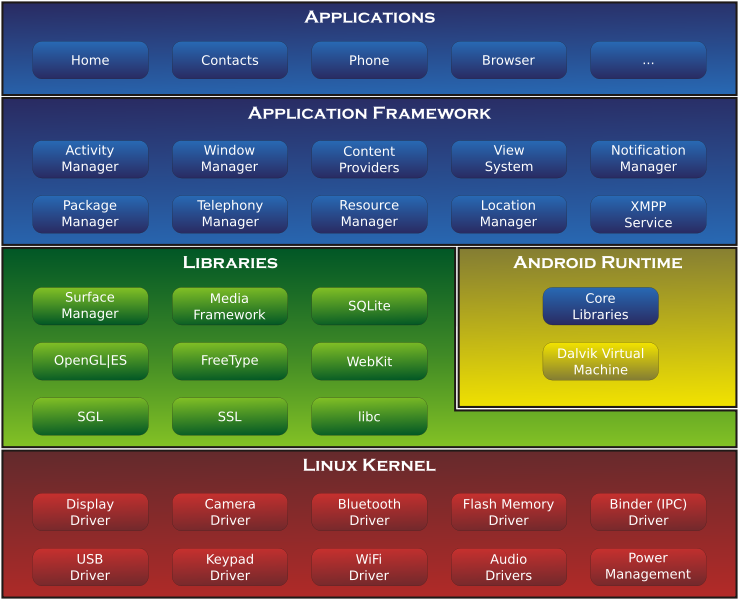
\includegraphics[scale=0.5]{android_architecture.png}
        \caption{Android Architecture}
        \label{fig:android_arch}
	\end{figure}
\subsection{Android Application Development:}    
	\subsection {Creating new project}
    	\begin{itemize}
			\item Open Android Studio
        	\item Select "Create new Android app"
	        \item Set minimum SDK version
	        \item Set the package name for the application
	        \item Select the starting $Activity$
	        \item Finish creating the project
		\end{itemize}  
    \subsection {Android Application Components}
        \begin{enumerate}
        	\item \textbf{Android Manifest}: All the components of the Android application are loosely coupled by the application manifest. It hat describes each component of the application and how they interact.
			\item \textbf{Activity}: An activity represents a single screen with a user interface,in-short Activity performs actions on the screen. For example, an email application might have one activity that shows a list of new emails.
            \item \textbf{Services}: A service is a component that runs in the background to perform long-running operations. For example, a service might play music in the background while the user is in a different application.
            \item \textbf{Broadcast Receivers}: Broadcast Receivers simply respond to broadcast messages from other applications or from the system. For example, applications can also initiate broadcasts to let other applications know that some data has been downloaded to the device and is available for them to use, so this is broadcast receiver who will intercept this communication and will initiate appropriate action.
            \item \textbf{Content Providers}: A content provider component supplies data from one application to others on request. The data may be stored in the file system, the database or somewhere else entirely.
		\end{enumerate} 
        
\subsection{Android - Phone Call}
	Android provides built-in APIs for phone calls.
    \begin{enumerate}
    \item \textbf{Action to make Phone Call}:
     You will use $ACTION\_CALL$ action to trigger built-in phone call functionality available in Android device. Following is simple syntax to create an intent with $ACTION\_CALL$ action.
     	\begin{lstlisting}
     		Intent phoneIntent = new Intent(Intent.ACTION_CALL);
     	\end{lstlisting}
     \item \textbf{ Data/Type to make Phone Call}:
     To make a phone call at a given number 91-000-000-0000, you need to specify tel: as URI using setData() method as follows −
     
     	\begin{lstlisting}
     		phoneIntent.setData(Uri.parse("tel:91-000-000-0000"));
     	\end{lstlisting}
        
    \item \textbf{Uri}:
    Creates a Uri object, using the string passed to it; the fact that the string is parsed to do this is completely hidden from the user.
     Uri object is in turn an immutable reference to a URI. This Uri object is then used in any Android API requiring a Uri object. When the reference does not have to be mutable, it can be used wherever a URI is expected too.
	\end{enumerate}
    
\subsection{Shared Preferences}     
Android provides many ways of storing data of an application. One of this way is called Shared Preferences. Shared Preferences allow you to save and retrieve data in the form of key, value pair.

In order to use shared preferences, you have to call a method $getSharedPreferences()$ that returns a $SharedPreference$ instance pointing to the file that contains the values of preferences.\\
	\begin{lstlisting}
SharedPreferences sharedpreferences = getSharedPreferences("pref_file", MODE);	
	\end{lstlisting}
The first parameter is the key and the second parameter is the MODE.
 	
\section{Outcomes :}
The source code of the Android Application developed to perform emergency call is Open-Source and available on GitHub at \url{https://github.com/AkshayChordiya/EmergencyCall}


\section{Testing :}

\subsection {Positive / Negative Testing}

\textbf{Positive Testing :}\\
If the entered number is a valid number then make the call.\\
Example- Input: "9000011111" \\
		 Output: true\\

\textbf{ Negative Testing :}\\
If the entered number is invalid number then calling fails.\\
Example- Input: "9001" \\
		 Output: false\\

\section{Conclusion : }

We have successfully developed a Smart Android Mobile Application to perform emergency land-line number/ mobile number calls


\end{document}
 
